\documentclass[border=5pt]{standalone}
\usepackage{pgfplots}
\pgfplotsset{compat=1.18}
\usepackage{siunitx}
\usepackage{tikz}
\usetikzlibrary{calc}

\definecolor{trainColor}{RGB}{31,119,180}
\definecolor{valColor}{RGB}{255,127,14}

\begin{document}
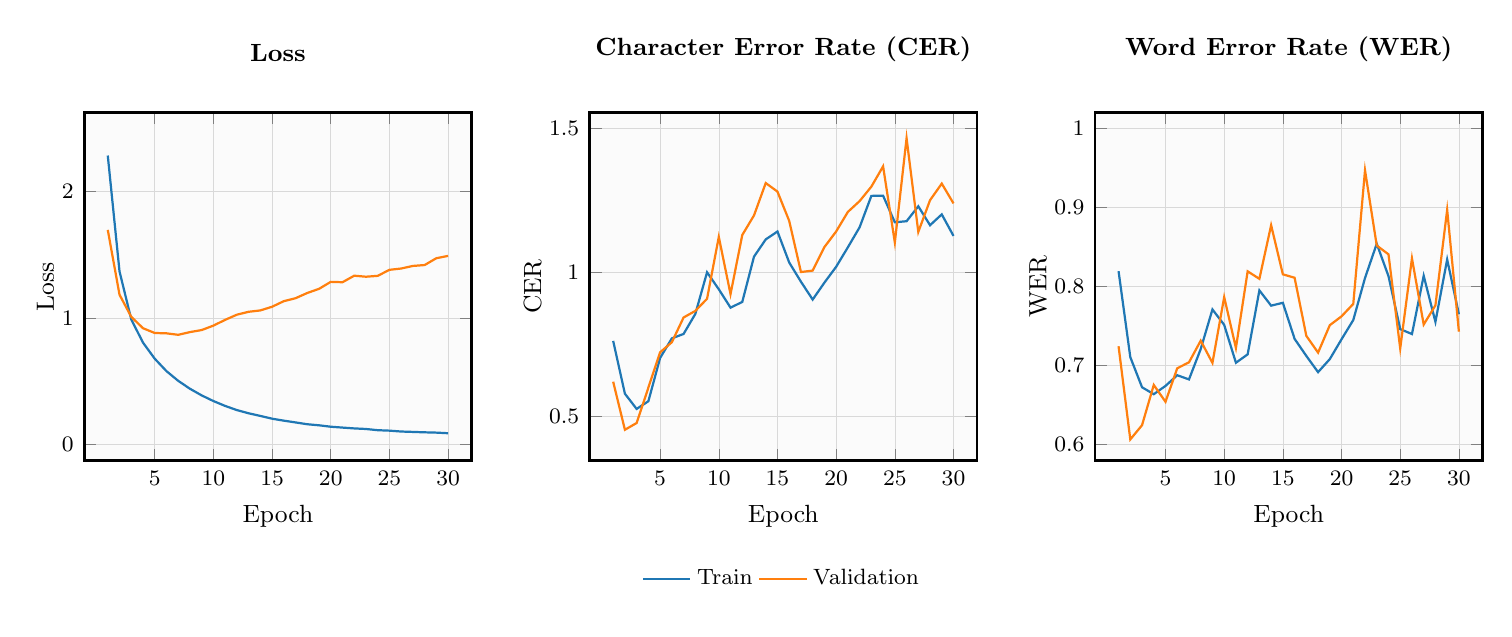
\begin{tikzpicture}[remember picture]

    % Graph 1: Loss
    \begin{axis}[
        name=plot1,
        width=6.5cm,
        height=6cm,
        xlabel={Epoch},
        ylabel={Loss},
        ylabel style={yshift=-0.15cm},
        xmin=0.5, xmax=30.5,
        ymin=0, ymax=2.5,
        xtick={5,10,15,20,25,30},
        grid=both,
        grid style={line width=.1pt, draw=gray!10},
        major grid style={line width=.2pt,draw=gray!30},
        title={Loss},
        axis background/.style={fill=gray!3},
        title style={yshift=3mm, font=\small\bfseries},
        label style={font=\small},
        tick label style={font=\footnotesize},
        line width=1pt,
        enlarge x limits=0.05,
        enlarge y limits=0.05,
        every axis plot/.append style={no markers},
        legend to name=commonlegend,
        legend columns=2,
        legend style={draw=none, fill=none, font=\footnotesize}
    ]
        % Train
        \addplot[color=trainColor, thick] coordinates {
            (1, 2.2859) (2, 1.3702) (3, 0.9906) (4, 0.8073) (5, 0.6801)
            (6, 0.5818) (7, 0.5052) (8, 0.4426) (9, 0.3900) (10, 0.3453)
            (11, 0.3067) (12, 0.2739) (13, 0.2486) (14, 0.2277) (15, 0.2059)
            (16, 0.1903) (17, 0.1763) (18, 0.1619) (19, 0.1536) (20, 0.1423)
            (21, 0.1355) (22, 0.1290) (23, 0.1245) (24, 0.1149) (25, 0.1113)
            (26, 0.1044) (27, 0.1013) (28, 0.0981) (29, 0.0957) (30, 0.0909)
        };
        
        % Validation
        \addplot[color=valColor, thick] coordinates {
            (1, 1.6979) (2, 1.1859) (3, 1.0111) (4, 0.9210) (5, 0.8832)
            (6, 0.8806) (7, 0.8688) (8, 0.8903) (9, 0.9065) (10, 0.9415)
            (11, 0.9871) (12, 1.0279) (13, 1.0508) (14, 1.0616) (15, 1.0906)
            (16, 1.1348) (17, 1.1581) (18, 1.1995) (19, 1.2322) (20, 1.2874)
            (21, 1.2845) (22, 1.3361) (23, 1.3280) (24, 1.3349) (25, 1.3826)
            (26, 1.3929) (27, 1.4133) (28, 1.4203) (29, 1.4744) (30, 1.4928)
        };
        
        \legend{Train, Validation}
    \end{axis}
    
    % Graph 2: CER, positioned to the right of plot1
    \begin{axis}[
        name=plot2,
        at={($(plot1.east)+(1.5cm,0)$)},
        anchor=west,
        width=6.5cm,
        height=6cm,
        xlabel={Epoch},
        ylabel={CER},
        ylabel style={yshift=-0.15cm},
        xmin=0.5, xmax=30.5,
        ymin=0.4, ymax=1.5,
        xtick={5,10,15,20,25,30},
        grid=both,
        grid style={line width=.1pt, draw=gray!10},
        major grid style={line width=.2pt,draw=gray!30},
        title={Character Error Rate (CER)},
        axis background/.style={fill=gray!3},
        title style={yshift=3mm, font=\small\bfseries},
        label style={font=\small},
        tick label style={font=\footnotesize},
        line width=1pt,
        enlarge x limits=0.05,
        enlarge y limits=0.05,
        every axis plot/.append style={no markers}
    ]
        % Train
        \addplot[color=trainColor, thick] coordinates {
            (1, 0.7611) (2, 0.5775) (3, 0.5245) (4, 0.5514) (5, 0.7019)
            (6, 0.7699) (7, 0.7853) (8, 0.8549) (9, 0.9997) (10, 0.9407)
            (11, 0.8768) (12, 0.8966) (13, 1.0542) (14, 1.1141) (15, 1.1416)
            (16, 1.0338) (17, 0.9670) (18, 0.9049) (19, 0.9638) (20, 1.0189)
            (21, 1.0868) (22, 1.1564) (23, 1.2655) (24, 1.2661) (25, 1.1736)
            (26, 1.1774) (27, 1.2293) (28, 1.1635) (29, 1.2012) (30, 1.1262)
        };
        
        % Validation
        \addplot[color=valColor, thick] coordinates {
            (1, 0.6192) (2, 0.4521) (3, 0.4756) (4, 0.5987) (5, 0.7214)
            (6, 0.7565) (7, 0.8426) (8, 0.8654) (9, 0.9077) (10, 1.1228)
            (11, 0.9237) (12, 1.1294) (13, 1.1976) (14, 1.3101) (15, 1.2804)
            (16, 1.1784) (17, 1.0007) (18, 1.0056) (19, 1.0874) (20, 1.1417)
            (21, 1.2098) (22, 1.2474) (23, 1.2976) (24, 1.3682) (25, 1.1035)
            (26, 1.4660) (27, 1.1402) (28, 1.2505) (29, 1.3082) (30, 1.2393)
        };
    \end{axis}
    
    % Graph 3: WER, positioned to the right of plot2
    \begin{axis}[
        name=plot3,
        at={($(plot2.east)+(1.5cm,0)$)},
        anchor=west,
        width=6.5cm,
        height=6cm,
        xlabel={Epoch},
        ylabel={WER},
        ylabel style={yshift=-0.15cm},
        xmin=0.5, xmax=30.5,
        ymin=0.6, ymax=1.0,
        xtick={5,10,15,20,25,30},
        grid=both,
        grid style={line width=.1pt, draw=gray!10},
        major grid style={line width=.2pt,draw=gray!30},
        title={Word Error Rate (WER)},
        axis background/.style={fill=gray!3},
        title style={yshift=3mm, font=\small\bfseries},
        label style={font=\small},
        tick label style={font=\footnotesize},
        line width=1pt,
        enlarge x limits=0.05,
        enlarge y limits=0.05,
        every axis plot/.append style={no markers}
    ]
        % Train
        \addplot[color=trainColor, thick] coordinates {
            (1, 0.8195) (2, 0.7108) (3, 0.6727) (4, 0.6639) (5, 0.6744)
            (6, 0.6879) (7, 0.6826) (8, 0.7210) (9, 0.7711) (10, 0.7516)
            (11, 0.7037) (12, 0.7143) (13, 0.7952) (14, 0.7759) (15, 0.7795)
            (16, 0.7339) (17, 0.7123) (18, 0.6918) (19, 0.7083) (20, 0.7334)
            (21, 0.7577) (22, 0.8109) (23, 0.8542) (24, 0.8132) (25, 0.7462)
            (26, 0.7400) (27, 0.8136) (28, 0.7554) (29, 0.8343) (30, 0.7650)
        };
        
        % Validation
        \addplot[color=valColor, thick] coordinates {
            (1, 0.7246) (2, 0.6067) (3, 0.6247) (4, 0.6756) (5, 0.6543)
            (6, 0.6967) (7, 0.7042) (8, 0.7316) (9, 0.7035) (10, 0.7867)
            (11, 0.7224) (12, 0.8193) (13, 0.8098) (14, 0.8776) (15, 0.8155)
            (16, 0.8112) (17, 0.7377) (18, 0.7165) (19, 0.7512) (20, 0.7624)
            (21, 0.7781) (22, 0.9471) (23, 0.8519) (24, 0.8408) (25, 0.7218)
            (26, 0.8357) (27, 0.7520) (28, 0.7763) (29, 0.8971) (30, 0.7430)
        };
    \end{axis}

    % Positioning the common legend below all graphs
    \node at ($(plot1.south)!0.5!(plot3.south)+(0,-1.5cm)$) {\pgfplotslegendfromname{commonlegend}};
    
\end{tikzpicture}
\end{document}